\documentclass[12pt]{article}
\usepackage{../../preamble2}
\setenumerate{label=\Alph*,itemjoin={\quad},before={\mbox{}\bigskip\\},after={\bigskip\\}}
\usepackage{epigraph}

\title{UCLA Math Circle}
\author{James Toche (and family)}
\date{28 June 2020 \\(Last revision: \today)}

\begin{document}
\epigraph{An invitation to enjoy the beauty of mathematics with Professor Olga Radko}{}
\begin{minipage}{\textwidth}
\maketitle
\begin{abstract}
Notes on some problems from the UCLA Math Circle Intermediate-2 Assessment for Summer Session 2020. Comments and corrections welcome. 
\end{abstract}
\end{minipage}

\section*{1. Random Integer}
\begin{question}
Sarah chose a random integer between 1000 and 9999, inclusive. What is the probability that the integer is odd and all of its digits are distinct?
\begin{enumerate*}
  \item $\frac{14}{75}$
  \item $\frac{56}{225}$
  \item $\frac{107}{400}$
  \item $\frac{7}{25}$
  \item $\frac{9}{25}$
\end{enumerate*}
\end{question}

We are looking for
\begin{align*}
P = \frac{\text{Count of the odd integer with distinct digits}}{\text{Count of all possible integers}}
\end{align*}

The total number of possible $4$-digit integers is readily calculated. The first digit may be any natural except $0$ (because otherwise it would have fewer than $4$ digits), so that leaves a choice of $9$ integers. The second, third and fourth digits may be any of the $10$ integers from $0$ to $9$. 
\begin{align*}
\text{Count of all possible 4-digit integers} = 9 \times 10 \times 10 \times 10 = 9,000
\end{align*}

The number of ways to pick $4$ distinct integers to form a $4$-digit number is $9\times9\times8\times7=4,536$. It is also clear that half of these are odd, so the probability we are looking for is about $25.2\%$ ($2,268/9,000$) give or take a couple of percents. We have:
\begin{question}
\begin{enumerate*}
  \item $\frac{14}{75} \simeq 19\%$
  \item $\frac{56}{225} \simeq 25\%$
  \item $\frac{107}{400} \simeq 27\%$
  \item $\frac{7}{25} \simeq 28\%$
  \item $\frac{9}{25} \simeq 36\%$
\end{enumerate*}
\end{question}

Right away we can rule out answers A and E and we are particularly attracted to B. But let's do the math.

A $4$-digit integer may be represented by the $4$ boxes below, with the letters $a$, $b$, $c$, $d$ placeholders for the first, second, third, and fourth digits.

\begin{center}
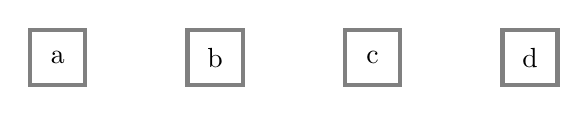
\begin{tikzpicture}[%
  node distance=2cm,
  nodestyle/.style={%
    rectangle,
    minimum width=2em,
    text centered,
    minimum height=2em,
    draw=black!50,
    ultra thick,
  }
]
  \node [nodestyle] (a) {a};
  \node [nodestyle, right of=a] (b) {b};
  \node [nodestyle, right of=b] (c) {c};
  \node [nodestyle, right of=c] (d) {d};
\end{tikzpicture}
\end{center}
with the following constraints:
\begin{align*}
a & \in \{1,2,3,4,5,6,7,8,9\} \\
b,c & \in \{0,1,2,3,4,5,6,7,8,9\} \\
d & \in \{1,3,5,7,9\} \\
\end{align*}
To randomly draw an odd number $abcd$ from $[1000,9999]$ is like drawing $a$ from $\{1,2,\ldots,9\}$, drawing $b,c$ from $\{0,1,\ldots,9\}$, with replacement, and drawing $d$ from $\{1,3,5,7,9\}$. Without the requirement of distinct digits, you could imagine drawing from the $4$ sets simultaneously. But the requirement of distinct digits puts a constraint on the drawing. You can no longer think of it as a simultaneous draw. But with some care, you can think of it as a sequential draw of the $4$ digits. 

Enforcing distinct digits can be done by imagining drawing without replacement. If you first pick the last digit, $d$, then whichever digit you draw is no longer ``available'' when you go on to draw, say, the second digit $b$. On the other hand, if you draw $b$ first, it may or may not impact the probability of drawing $d$. That is, if you draw a $0$ for $b$, you still have $5$ choices for $d$, but if you draw a $1$ for $b$, you are left with only $4$ choices for $d$. Similarly, if you draw a $0$ for the third digit, $c$, say, it still leaves $9$ choices for the first digit $a$, whereas if you draw a $1$, it leaves only $8$ choices for $a$. Thus, to get the calculation right, you have to imagine a predetermined order of digit selection that ``works''. These work:
\begin{align*}
& d \rightarrow a \rightarrow b \rightarrow c \\
& d \rightarrow a \rightarrow c \rightarrow b
\end{align*}
The section \textbf{Why Selection Order Matters} (below) goes over this point again. For now, consider a sequential draw $d \rightarrow a \rightarrow b \rightarrow c$. If you draw $d$ first ($5$ choices), that leaves one less digit for $a$ ($8$ choices), and subsequently one less digit for $b$ ($8$ choices), and lastly one less digit for $c$ ($7$ choices). And thus, the probability is:
\begin{align*}
P = \frac{5 \times 8 \times 8 \times 7}{9 \times 10 \times 10 \times 10} 
  = \frac{8 \times 7}{9 \times 5 \times 5} 
  = \frac{56}{225} 
  \simeq 24.9\%
\end{align*}

\fbox{The correct answer is B.} Our rough estimate of $25.2\%$, it turns out, was pretty accurate. 


\subsubsection*{Why Selection Order Matters}
Consider the problem of selecting a two-digit number with distinct digits taken from $\{0,1,2\}$. Here are all the two-digit combinations that can be formed:
\begin{align*}
00, 01, 02, 10, 11, 12, 20, 21, 22
\end{align*}
To keep only two-digit numbers, we remove $00$, $01$, and $02$. And to keep distinct digits, we remove $11$ and $22$. This leaves: 
\begin{align*}
\crossout[3]{00}, \crossout[3]{01}, \crossout[3]{02}, 
10, \crossout[3]{11}, 12, 20, 21, \crossout[3]{22}
\end{align*}
Thus $4$ numbers out of $9$ satisfy the criteria. 

How can we calculate this systematically? The total number of possibilities is $3$ choices for the first position and $3$ choices for the second position:
\begin{align*}
3 \times 3 = 9
\end{align*}
It helps to draw boxes to visualize the problem: we want to fill the boxes with the available digits, while satisfying the constraints of the problem.
\begin{center}
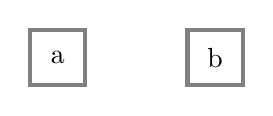
\begin{tikzpicture}[%
  node distance=2cm,
  nodestyle/.style={%
    rectangle,
    minimum width=2em,
    text centered,
    minimum height=2em,
    draw=black!50,
    ultra thick,
  }
]
  \node [nodestyle] (a) {a};
  \node [nodestyle, right of=a] (b) {b};
\end{tikzpicture}
\end{center}
Box $a$ stores the tens digit, while box $b$ stores the unit digit. We can think of the digits as being selected sequentially, either in order $a \rightarrow b$ or in order $b \rightarrow a$.

Case \fbox{$a \rightarrow b$} Suppose we select the tens digit first, followed by the unit digit. There are $2$ choices for the tens digit ($1$ and $2$, since $0$ is ruled out). Once the tens digit has been selected, there are only $2$ choices left for the unit digit ($3-1=2$), since one of the digits has been used already:
\begin{align*}
2 \times 2 = 4
\end{align*}
Case \fbox{$b \rightarrow a$} Suppose instead that we select the unit digit first, followed by the tens digit. There are $3$ choices for the unit digit ($0$, $1$, and $2$). Once the unit digit has been selected, how many choices for the tens digit? That depends. If the unit digit was $0$, we still have $2$ choices left for the tens digit ($1$ and $2$ are both still available), but if the unit digit was not $0$, then we have only one choice left for the tens digit (if the unit digit was $1$, that leaves only $2$ for the tens digit, while if the unit digit was $2$, that leaves only $1$ for the tens digit). Thus, if we select the unit digit first, followed by the tens digit, the correct calculation is:
\begin{align*}
3 \times \left(\frac{1}{3}\times2 + \frac{2}{3}\times1\right)
= 4
\end{align*}
We get the same answer, of course, but the calculation is more complicated.

Conclusion: it is much easier to calculate the cases if we select the tens digit before the unit digit. 


\newpage
\section*{2. No Sport Days!}
\begin{question}
John plays soccer once every three days, plays basketball once every four days and plays volleyball every five days. He played all three sports on December 31st, 2018. How many days in 2019 did John not play any of the sports?
\begin{enumerate*}
  \item $78$
  \item $146$
  \item $144$
  \item $80$
  \item $152$
\end{enumerate*}
\end{question}

It helps to visualize the problem with a timeline. Figure~\ref{fig:sports:timeline} shows the first $60$ days. A brute-force strategy would be to extend the timeline to $365$ days and count the days where John played no sports. But it would be nicer to find another method. Note that on day $60$, all three sports are played. In a sense, everything ``resets'' on day $60$: day $61$ is like $1$st January. Since $6\times 60=360$, days $361$ and $362$ are no-sport days to be added to six times the count from $1$ to $60$. Looking at the figure, we count $24$ within the $60$-day period and so the answer is:
\begin{align*}
6 \times 24 + 2 = 146
\end{align*}
\begin{figure}[hptb]
\begin{minipage}[b]{\textwidth}
\centering
\includegraphics[width=\textwidth]%
{sports-timeline}
\caption{\textbf{The first $60$ days}.
\label{fig:sports:timeline}}
\end{minipage}
\end{figure}

If you can sketch a timeline fast enough, this could be a reasonable approach. Is there a more subtle approach? It is obvious that there will be no sports on prime-number days greater than $5$. It often helps to have memorized a bunch of prime numbers. Here you would need to quickly figure out this list:
\begin{align*}
&7, 11, 13, 17, 19, 23, 29, 31, 37, 41, 43, 47, 53, 59, 61, 67, 71, 73, 79, 83, 89, 97, 101, 103, 107, 109, 113, 127, 131, 137, \\&139, 149, 151, 157, 163, 167, 173, 179, 181, 191, 193, 197, 199, 211, 223, 227, 229, 233, 239, 241, 251, 257, 263, 269, \\&271, 277, 281, 283, 293, 307, 311, 313, 317, 331, 337, 347, 349, 353, 359
\end{align*}
But even that wouldn't be enough, because numbers of the form $2p$, for $p$ prime, are also no-sports day. For instance, $14$. So are numbers of the form $p_{a} \times p_{b}$, for $p_{a},p_{b}$ prime. For instance $7 \times 11=77$.

Another strategy is, instead, to count all sports days and deduct from $365$. That is more manageable. To calculate how many multiples of $3$ there are in $365$, divide the nearest, smaller multiple of $3$: $363/3=121$ are all soccer days. For soccer, basketball, volleyball, one gets:
\begin{align*}
\frac{363}{3} & = 121 \\
\frac{364}{4} & = 91 \\
\frac{365}{5} & = 73 \\
\end{align*}
However, multiples of $3 \times 4=12$ have been counted twice. And so have multiples of $3 \times 5$ and $4 \times 5$. 
\begin{align*}
\frac{360}{12} & = 30 \\
\frac{360}{15} & = 24 \\
\frac{360}{20} & = 18 \\
\end{align*}
If we add up the first three numbers and subtract the last three, we are getting closer, but there is still one problem. Consider $3 \times 4 \times 5=60$. The number $60$ is included among the $121$ multiples of $3$, among the $91$ multiples of $4$, and among the $73$ multiples of $5$. It is also among the $30$ multiples of $12$, among the $24$ multiples of $15$, and among the $18$ multiples of $20$. Thus by adding and subtracting we have in effect removed all the multiples of $60$. Since $360/60=6$, we must add those $6$ back in. In total,
\begin{align*}
121 + 91 + 73 - 30 - 24 - 18 + 6 & = 219 \\
365 - 219 & = 146
\end{align*}
as we had found earlier by a direct counting method.

\fbox{The correct answer is B.}



\newpage
\section*{3. Congruent Circles and Angle}
\begin{question}
Two congruent circles centered at points $A$ and $B$ each pass through the other circle's center. The line containing both $A$ and $B$ is extended to intersect the circles at points $C$ and $D$. The circles intersect at two points, one of which is $E$. What is the degree measure of $\angle CED$?
\begin{enumerate*}
  \item $100^{\circ}$
  \item $120^{\circ}$
  \item $130^{\circ}$
  \item $135^{\circ}$
  \item $150^{\circ}$
\end{enumerate*}
\end{question}
Refer to the figures. Triangle $AEB$ is equilateral, so $\angle AEB=60^{\circ}$. Angle $\angle CAE$ is the complement of $\angle BAE$, so $\angle CAE=180-60=120^{\circ}$. Triangle $CAE$ is isosceles, so $\angle CEA=30^{\circ}$. Putting it together,
\begin{align*}
\angle CED 
  & = \angle CEA + \angle AEB + \angle BED \\
  & = 30^{\circ} + 60^{\circ} + 30^{\circ} \\
  & = 120^{\circ}
\end{align*}

\fbox{The correct answer is B.}

\begin{minipage}[b]{\textwidth}
\subsubsection*{Step~1: Draw the figure}
\centering
\includegraphics[width=\textwidth]%
{congruent-circles-1}
\end{minipage}

\begin{minipage}[b]{\textwidth}
\subsubsection*{Step~2: Identify common lengths}
\centering
\includegraphics[width=\textwidth]%
{congruent-circles-2}
\end{minipage}

\begin{minipage}[b]{\textwidth}
\subsubsection*{Step~3: Identify the equilateral triangle}
\centering
\includegraphics[width=\textwidth]%
{congruent-circles-3}
\end{minipage}

\begin{minipage}[b]{\textwidth}
\subsubsection*{Step~4: Identify the isosceles triangle}
\centering
\includegraphics[width=\textwidth]%
{congruent-circles-4}
\end{minipage}

\begin{minipage}[b]{\textwidth}
\subsubsection*{Step~5: Putting it together}
\centering
\includegraphics[width=\textwidth]%
{congruent-circles-5}
\end{minipage}


\newpage
\section*{4. Semi-Circle Inscribed in Triangle}
\begin{question}
A semicircle is inscribed in an isosceles triangle with base $16$ and height $15$ so that the diameter of the semicircle is contained in the base of the triangle as shown. What is the radius of the semicircle?
\begin{center}
\includegraphics[height=0.2\textheight]%
{semi-circle-triangle-1}
\end{center}
\begin{enumerate*}
  \item $4\sqrt{3}$
  \item $17\sqrt{2}$
  \item $17\sqrt{3}$
  \item $10$
  \item $\frac{120}{17}$
\end{enumerate*}
\end{question}


\subsubsection*{Approach I: Area of Triangle}
Refer to Figure~\ref{fig:semi:circle:triangle:1}.
\begin{figure}[hptb]
\begin{minipage}[b]{\textwidth}
\centering
\includegraphics[height=0.4\textheight]%
{semi-circle-triangle-2}
\caption{\label{fig:semi:circle:triangle:1}}
\end{minipage}
\end{figure}
The known lengths are $AB=15$ and $BC=8$. Applying Pythagoras to $ABC$ yields:
\begin{align*}
AC = \sqrt{15^2 + 8^2} = \sqrt{289} = 17
\end{align*}
The area of triangle $ABC$ is given by the formula $(1/2)\times \text{height}\times\text{base}$:
\begin{align*}
\text{Area of}~ABC 
  = \frac{BD \times AC}{2} 
  = \frac{17r}{2} 
\end{align*}

Another way to compute this area is to consider $ABC$ as half of a rectangle:
\begin{align*}
\text{Area of}~ABC 
  = \frac{AB \times BC}{2} 
  = \frac{15 \times 8}{2} 
\end{align*}

Equating the two expressions gives:
\begin{align*}
\frac{17r}{2} & = \frac{15 \times 8}{2}  \\
r & = \frac{120}{17}
\end{align*}

\fbox{The correct answer is E.}

\clearpage
\subsubsection*{Approach II: Pythagoras \& System of Equations}
The approach detailed here was our first attempt. It is unnecessarily complicated. 
\begin{figure}[hptb]
\begin{minipage}[b]{\textwidth}
\centering
\includegraphics[height=0.4\textheight]%
{semi-circle-triangle-3}
\caption{\label{fig:semi:circle:triangle:2}}
\end{minipage}
\end{figure}


Refer to Figure~\ref{fig:semi:circle:triangle:2}. Triangles $ADB$ and $BDC$ are right-angled, i.e. $\angle ADB=90^{\circ}$ and $\angle BDC=90\circ$. We have seen earlier that $AC=17$ follows from an application of the Pythagoras relation to triangle $ABC$. Applying Pythagoras to $ADB$ yields:
\begin{align*}
(17-x)^2 + r^2 = 15^2
\end{align*}
Applying Pythagoras to $BDC$ yields:
\begin{align*}
r^2 + x^2 = 8^2
\end{align*}
Subtracting the last two equations yields:
\begin{align*}
(17-x)^2 - x^2 & = 15^2 - 8^2 \\
17^2 - 2 \cdot 17 \cdot x + x^2 - x^2 & = 15^2 - 8^2 \\
x & = \frac{17^2 - 15^2 + 8^2}{2 \cdot 17} \\
\end{align*}
which we can use in $r^2=8^2-x^2$:
\begin{align*}
r^2 & = 8^2 - \left(\frac{17^2 - 15^2 + 8^2}{2 \cdot 17}\right)^2 \\
& = 64 - \left(\frac{289 - 225 + 64}{2 \cdot 17}\right)^2 \\
& = 64 - \left(\frac{64}{17}\right)^2 \\
& = \frac{64 \cdot 17^2 - 64^2}{17^2} \\
& = \frac{64(289-64)}{17^2} \\
& = \frac{64 \cdot 225}{17^2} \\
& = \frac{8^2 \cdot 15^2}{17^2} \\
\implies \hspace{2em}
r = \sqrt{r^2} & = \frac{8 \cdot 15}{17} \\
  & = \frac{120}{17}
\end{align*}

\fbox{The correct answer is E.}

This was a long and tedious calculation. There may be a shorter way \ldots [Update: There is a shorter way! See the previous section.]





\newpage
\section*{5. Ordering Big Numbers}
\begin{question}
What is the correct ordering of the three numbers $10^{8}$, $5^{12}$, and $2^{24}$.
\begin{enumerate*}
  \item $2^{24} < 10^{8} < 5^{12}$
  \item $2^{24} < 5^{12} < 10^{8}$
  \item $5^{12} < 2^{24} < 10^{8}$
  \item $10^{8} < 5^{12} < 2^{24}$
  \item $10^{8} < 2^{24} < 5^{12}$
\end{enumerate*}
\end{question}

We have $10 = 2 \times 5$, so we can rewrite $10^{8}$ in terms of $2^{24}$ and $5^{12}$ and check whether the multiplier is greater or smaller than $1$.
\begin{align*}
10^{8} & = 5^{8}2^{-16} \times 2^{24} \\
       & = \left(\frac{5}{4}\right)^{8} \times 2^{24} \\
       & > \hspace{3.9em} 2^{24}
\end{align*}
since $\frac{5}{4}>1$ (any number greater than $1$ raised to some positive power is greater than $1$). 

Similarly,
\begin{align*}
10^{8} & = 2^{8}5^{-4} \times 5^{12} \\
       & = \left(\frac{4}{5}\right)^{4} \times 5^{12} \\
       & < \hspace{3.9em} 5^{12}
\end{align*}
since $\frac{5}{4}<1$ (the inverse of the fraction above). 


Putting it together,
\begin{align*}
2^{24} < 10^{8} < 5^{12}
\end{align*}

\fbox{The correct answer is A.}

A trick we learned at the \textit{UCLA Math Cirle} that simplifies the problem is to note that the exponents are all multiples of $4$:
\begin{align*}
 8 & = 2 \times 4 \\
12 & = 3 \times 4 \\
24 & = 6 \times 4
\end{align*}
For any $0<a<b$, we have
\begin{align*}
0 < a < b
~\Longleftrightarrow~
0 < a^4 < b^4
\end{align*}
Thus the question reduces to comparing $10^{2}=100$, $5^{3}=125$, and $2^{6}=64$, which is straightforward!



\newpage
\section*{6. Moduli}
\begin{question}
What is the tens digit of $7^{2011}$ 
\begin{enumerate*}
  \item $0$
  \item $1$
  \item $3$
  \item $4$
  \item $7$
\end{enumerate*}
\end{question}

If you have access to a computer/calculator, you can make the following table. However, try $7^{2011}$ and it most likely will give you either an error or something like \texttt{Inf}. That is because the number $7^{2011}$ is large beyond imagination. The largest power of $7$ we were able to compute/estimate was $7^{364} \simeq 4.1 \times 10^{307}$, which doesn't help with the tens digit!
\begin{center}
\renewcommand{\arraystretch}{1.5}
\newcolumntype{C}[1]{>{\centering\arraybackslash}p{#1}} % centered 'p' col.
\begin{tabular}{*{3}{C{0.17\linewidth}}}
    \hline
    Exponent  &  Number &  $10$-Digit \\
    \hline
    $0$  &  $1$ &  $0$ \\
    $1$  &  $7$ &  $0$ \\
    $2$  &  $49$ &  $4$ \\
    $3$  &  $343$ &  $4$ \\
    $4$  &  $2,401$ &  $0$ \\
    $5$  &  $16,807$ &  $0$ \\
    $6$  &  $117,649$ &  $4$ \\
    $7$  &  $823,543$ &  $4$ \\
    $8$  &  $5,764,801$ &  $0$ \\
    $9$  &  $40,353,607$ &  $0$ \\
    \hline
    \end{tabular}
\end{center}
without a calculator and no special tricks, the largest powers we can compute are the first $5$ or $6$. It's a bit of a stretch from that to guess that the tens digits come in sequences of $0,0,4,4,0,0,4,4,\ldots$ At this point, you're faced with a toss-up between $0$ and $4$ or you can work out whether $2011$ maps to exponent $0$, $1$, $2$, or $3$.

\begin{definition*}[Modular Arithmetic]
\begin{align*}
a\Mod{b} = \texttt{remainder of}~a/b
\end{align*}
\end{definition*}
In general, we have $a\Mod{b}\in[0,b-1]$. For instance, 
\begin{align*}
11\Mod{3} \equiv 2
\end{align*}
which may be read ``eleven mod three is congruent to two.'' The word comes from the latin ``modulus'', whose plural form is ``moduli.'' 

An analogy to give intuition about modular arithmetic is the hour system. Some countries in Europe use a $24$ hour clock, while other countries like the United States more commonly use a $12$ hour clock (except the military, who also use the $24$ hour clock!). Thus $8{:}00$pm would be equivalent to $20{:}00$ (In France, the popular evening news slot is called ``the twenty-hour'' --- ``le vingt-heure''). In modular arithmetic, that is
\begin{align*}
20\Mod{12} \equiv 8
\end{align*}

We all do modular arithmetic without thinking (too hard). For instance, if it takes about $50$ hours to watch all James Bond movies, what time will it be when you finish, if you start at $10$pm? The answer is midnight because
\begin{align*}
50\Mod{24} \equiv 2
\end{align*}

In \texttt{Python} and the \texttt{C} languages, the \texttt{mod} command is the percentage sign. A typical command is the first line, a typical return is the second line:
\begin{align*}
& \texttt{50 \% 24}\\
& \texttt{2}
\end{align*}
You can check this calculation in an online \texttt{Python} emulator. There are online modulo calculators that you can play with too.

From the pattern detected above, it is clear that $7^{n}$ has a tens digit of $0$ whenever $n$ is a multiple of $4$. A candidate for a multiple of $4$ near $2011$ is $2010$, but it is easily verified that it's not a multiple of $4$. It follows immediately that $2008$ is a multiple of $4$, which can also be verified easily by dividing by $2$ twice. To sum up,
\begin{center}
\renewcommand{\arraystretch}{1.5}
\newcolumntype{C}[1]{>{\centering\arraybackslash}p{#1}} % centered 'p' col.
\begin{tabular}{*{5}{C{0.17\linewidth}}}
  \toprule
  ten digit $=$
    &     $0$ &     $0$ &    $4$ & \circletext{$4$} \\
  \midrule
  modulo value $=$ 
    &     $0$ &     $1$ &   $2$  & \circletext{$3$}\\
    &  \ldots &  \ldots &              \ldots &  \ldots \\
  other values of $n$ 
    &  $2004$ &  $2005$ &              $2006$ &  $2007$ \\
    &  $2008$ &  $2009$ & $2010$ & \circletext{$2011$} \\
    &  $2012$ &  $2013$ & $2014$ & $2015$ \\
  \bottomrule
  \end{tabular}
\renewcommand{\arraystretch}{1}
\end{center}
In \texttt{mod} notation,
\begin{align*}
7^{2008}\Mod{4} \equiv 0 \\
7^{2011}\Mod{4} \equiv 3
\end{align*}
which implies that the digit is $4$. 

\fbox{The correct answer is D.}

\newpage
\section*{7. Area of Triangle in Cartesian Coordinates}
\begin{question}
What is the area of the triangle with vertices $A=(1,3)$, $B=(5,1)$, $C=(4,4)$.
\begin{enumerate*}
  \item $5$
  \item $3\sqrt{2}$
  \item $\frac{4}{3}\sqrt{2}$
  \item $3\sqrt{3}$
  \item $6$
\end{enumerate*}
\end{question}

\begin{figure}[hptb]
\begin{minipage}[b]{\textwidth}
\centering
\includegraphics[height=0.5\textheight]%
{triangle-cartesian-area}
\caption{\textbf{Area of Triangle in a Cartesian Coordinate System}.
\label{fig:triangle:cartesian:area}}
\end{minipage}
\end{figure}

Refer to Figure~\ref{fig:triangle:cartesian:area}. Before you draw a figure in a Cartesian coordinate system, check the largest and smallest values for each axis, to ensure that your figure will fit. Here all the coordinates are positive, ranging on $[1,5]$ on $x$ and $[1,4]$ on $y$. Since $1$ is close enough to $0$, we will include the origin and, for symmetry, we'll set the limits to $[0,5]$ along both axes. 

With an accurately drawn triangle, a few properties are immediately apparent. (1)~The triangle is isosceles: length $CA$ equals length $CB$. To see this, note that length $CA$ spans three units horizontally for one unit vertically, while length $CB$ spans three units vertically for one unit horizontally. (2)~The angle $\angle ACB$ is a right angle. This can be seen by rotating the triangle around point $C$, moving point $A$ by one unit vertically and point $B$ by one unit horizontally. Once you see this, you also see that the area of the triangle is a little more than half of $3 \times 3$, since the lengths $CA$ and $CB$ are a little longer than $3$. So we are looking for an area approximately equal to $5$. 

It pays to know that $\sqrt{2}\simeq1.414$ and $\sqrt{3}\simeq1.732$. From this we have the approximations: 
\begin{question}
\begin{enumerate*}
  \item $5$
  \item $3\sqrt{2}\simeq 4.24$
  \item $\frac{4}{3}\sqrt{2} \simeq 1.89$
  \item $3\sqrt{3} \simeq 5.20$
  \item $6$
\end{enumerate*}
\end{question}
From this, we can rule out $B$, $C$, $E$. We lean towards A, but let's do the math. We can apply Pythagoras. 

Length $AC$ may be computed from the triangle formed by points $A$, $(1,4)$, and $C$:
\begin{align*}
AC^2 = (4-1)^2 + (4-3)^2 = 10
\end{align*}

Length $CB$ may be computed from the triangle formed by points $C$, $(5,4)$, and $B$.
\begin{align*}
CB^2 = (5-4)^2 + (4-1)^2 = 10
\end{align*}

Length $AB$ may be computed from the triangle formed by points $A$, $(1,1)$, and $B$.
\begin{align*}
AB^2 = (3-1)^2 + (5-1)^2 = 20
\end{align*}

We can verify that the angle is a right angle by checking the Pythagoras relation:
\begin{align*}
(\sqrt{10})^2 + (\sqrt{10})^2  = 20 = (\sqrt{20})^2 
\end{align*}

Finally, the area is given by:
\begin{align*}
\frac{1}{2} \sqrt{10} \times \sqrt{10}  = 5
\end{align*}
as we suspected. 

\fbox{The correct answer is A.}



\newpage
\section*{8. A Quartic Equation!}
\begin{question}
How many different real numbers satisfy the equation $(x^2-5)^2=16$~?
\begin{enumerate*}
  \item $0$
  \item $1$
  \item $2$
  \item $4$
  \item $8$
\end{enumerate*}
\end{question}
This is a polynomial of degree $4$ since $(x^2-5)^2=x^4-10x^2+25$. This is also called a quartic equation. 
\begin{theorem*}[Fundamental Theorem of Algebra]
Every polynomial of degree $n$ with complex coefficients has exactly $n$ complex roots. That is, every equation of the form
\begin{align*}
a_{n}x^{n} + a_{n-1}x^{n-1} + \ldots + a_{2}x^{2} + a_{1}x^{1} + a_{0}x^{0}
= 0,
\end{align*}
with $a_{n}\neq 0$, has exactly $n$ roots. There is a catch: roots are counted with multiplicity. Example: The polynomial $x^2=0$ has two roots, $0$ and $0$. 
\end{theorem*}
The Fundamental Theorem of Algebra implies that we can rule out answer E, because there can be at most $4$ distinct real roots. 
\begin{theorem*}[Complex Conjugate Root Theorem]
If a polynomial with real coefficients has a complex root $a+bi$ ($a$ and $b$ are real numbers, with $b\neq0$, and $i$ is the imaginary unit), then the complex conjugate $a-bi$ is also a root. In short, \textbf{complex roots come in pairs.}
\end{theorem*}
It follows that if the degree of a real polynomial is odd, it must have at least one real root. Since the polynomial has degree $4$, it may have $0$, $2$ or $4$ complex roots, implying that we can rule out answer B. 

The above considerations become automatic once you are familiar with polynomials. Moreover inspection immediately suggests the existence of two real roots, $1$ and $-1$. So now the remaining possibilities are C and D. 
In this example, we can actually solve the quartic equation by reducing it to a pair of quadratic equations: 
\begin{align*}
(x^2-5)^2 & = 16 
\Longrightarrow
  \begin{cases}
  ~~(x^2-5) = 4 
    \implies x^2 = 9
      \implies 
        \begin{cases}
        x = 3 \\
        x = -3
        \end{cases} \\ \\
  -(x^2-5) = 4 
    \implies x^2 = 1
      \implies 
        \begin{cases}
        x = 1 \\
        x = -1
        \end{cases} \\
  \end{cases} 
\end{align*}
So there are $4$ real roots. 

\fbox{The correct answer is D.}



\newpage
\section*{9. Sharing Markers}
\begin{question}
Ann has $24$ markers. In how many ways can she share them with Bob and Chris so that each of the three has at least two markers?
\begin{enumerate*}
  \item $105$
  \item $114$
  \item $190$
  \item $210$
  \item $380$
\end{enumerate*}
\end{question}

If Ann, Bob, and Chris each have $2$ markers, there remain $18$ to share among all three. How can exactly $18$ markers be split in $3$ groups? One way to understand the math behind this is to first analyze simpler problems. And pictures (mental visualizations or scribbles) help see what divisions are possible. The ``stars and bars'' visualization is useful in cases where a fixed number of objects (stars) are split into groups (by bars). The bars are dividers that can be placed between stars to form groups of different sizes. For $k$ groups, $k-1$ dividers are needed (one less). Thus, to divide $18$ stars into $3$ groups, only $2$ bars are needed.  

How can $1$ marker be split in $3$ groups? In the language of the stars-and-bars: How many ways can $1$ star and $2$ bars be arranged? Answer: $3$ ways. In simple cases, the stars-and-bars representation is immediate. And yes, you can place two bars next to each other and at the extremities too. 
\begin{figure}[hptb]
\begin{minipage}[b]{\textwidth}
\centering
\begin{tikzpicture}[framed]
  \def\total{1} % i+j+k = total
  \xdef\y{0}
  \foreach \i in {0,...,\total}{
    \pgfmathsetmacro{\maxj}{int(\total-\i)}
    \foreach \j in {0,...,\maxj}{
      \pgfmathparse{int(\y+1)}\xdef\y{\pgfmathresult}
      \pgfmathsetmacro{\k}{int(\total-\i-\j)}
      \foreach \i in {1,...,\total}
        \node at (\i,\y){$\star$};
      \node at (.45+\j+\i,\y) {$\big|$};
      \node at (.55+\i,\y) {$\big|$};
      \node[left] at (-1,\y){(\i,\j,\k)};
    }
  }
\end{tikzpicture}
\caption{\textbf{Stars and Bars: $1$ star and $2$ bars}.
\label{fig:stars:bars:1}}
\end{minipage}
\end{figure}

How can $2$ markers be split in $3$ groups? How many ways can $2$ stars and $2$ bars be arranged? Answer: $6$. Easy to visualize mentally.
\begin{figure}[hptb]
\begin{minipage}[b]{\textwidth}
\centering
\begin{tikzpicture}[framed]
  \def\total{2} % i+j+k = total
  \xdef\y{0}
  \foreach \i in {0,...,\total}{
    \pgfmathsetmacro{\maxj}{int(\total-\i)}
    \foreach \j in {0,...,\maxj}{
      \pgfmathparse{int(\y+1)}\xdef\y{\pgfmathresult}
      \pgfmathsetmacro{\k}{int(\total-\i-\j)}
      \foreach \i in {1,...,\total}
        \node at (\i,\y){$\star$};
      \node at (.45+\j+\i,\y) {$\big|$};
      \node at (.55+\i,\y) {$\big|$};
      \node[left] at (-1,\y){(\i,\j,\k)};
    }
  }
\end{tikzpicture}
\caption{\textbf{Stars and Bars: $2$ stars and $2$ bars}.
\label{fig:stars:bars:2}}
\end{minipage}
\end{figure}


\clearpage
How can $3$ markers be split in $3$ groups? That is, How many ways can $3$ stars and $2$ bars be arranged? Answer: $10$. This one may be a little harder to visualize without pen and paper. But you can still count the cases with your fingers. There are $3$ ways to have $(3,0,0)$. There are $6$ ways to have $(2,1,0)$. There is $1$ way to have $(1,1,1)$.
\begin{figure}[hptb]
\begin{minipage}[b]{\textwidth}
\centering
\begin{tikzpicture}[framed]
  \def\total{3} % i+j+k = total
  \xdef\y{0}
  \foreach \i in {0,...,\total}{
    \pgfmathsetmacro{\maxj}{int(\total-\i)}
    \foreach \j in {0,...,\maxj}{
      \pgfmathparse{int(\y+1)}\xdef\y{\pgfmathresult}
      \pgfmathsetmacro{\k}{int(\total-\i-\j)}
      \foreach \i in {1,...,\total}
        \node at (\i,\y){$\star$};
      \node at (.45+\j+\i,\y) {$\big|$};
      \node at (.55+\i,\y) {$\big|$};
      \node[left] at (-1,\y){(\i,\j,\k)};
    }
  }
\end{tikzpicture}
\caption{\textbf{Stars and Bars: $3$ stars and $2$ bars}.
\label{fig:stars:bars:3}}
\end{minipage}
\end{figure}


\clearpage
How can $4$ markers be split in $3$ groups? Answer: $15$.
\begin{figure}[hptb]
\begin{minipage}[b]{\textwidth}
\centering
\begin{tikzpicture}[framed]
  \def\total{4} % i+j+k = total
  \xdef\y{0}
  \foreach \i in {0,...,\total}{
    \pgfmathsetmacro{\maxj}{int(\total-\i)}
    \foreach \j in {0,...,\maxj}{
      \pgfmathparse{int(\y+1)}\xdef\y{\pgfmathresult}
      \pgfmathsetmacro{\k}{int(\total-\i-\j)}
      \foreach \i in {1,...,\total}
        \node at (\i,\y){$\star$};
      \node at (.45+\j+\i,\y) {$\big|$};
      \node at (.55+\i,\y) {$\big|$};
      \node[left] at (-1,\y){(\i,\j,\k)};
    }
  }
\end{tikzpicture}
\caption{\textbf{Stars and Bars: $4$ stars and $2$ bars}.
\label{fig:stars:bars:4}}
\end{minipage}
\end{figure}


\subsubsection*{General Case}
The mathematical formula associated with $s$ stars and $b$ bars is:
\begin{align*}
\binom{s + b}{b} = \frac{(s+b)!}{b!\,s!}
\end{align*}
And so for $s=18$ and $b=2$,
\begin{align*}
\binom{18 + 2}{2} 
  = \frac{20!}{18!\,2!} 
  = \frac{20 \times 19}{2} 
  = 190 
\end{align*}

\fbox{The correct answer is C.}

\clearpage
The case of $18$ markers would take up a lot of space to represent graphically. However, you can generate one with special software. Here are the first few lines:
\begin{figure}[hptb]
\begin{minipage}[b]{\textwidth}
\centering
\fbox{\includegraphics[trim=0 115cm 0 0,clip]%
{stars-and-bars-18}}
\caption{\textbf{Stars and Bars: $18$ stars and $2$ bars (only a few cases displayed)}.
\label{fig:stars:bars:18:cropped}}
\end{minipage}
\end{figure}


\clearpage
\section*{10. Shopping for Socks}
\begin{question}
Ralph went to the store and bought $12$ pairs of socks for a total of $\$24$. Some of the socks he bought cost $\$1$ a pair, some of the socks he bought cost $\$3$ a pair, and some of the socks he bought cost $\$4$ a pair. If he bought at least one pair of each type, how many pairs of $\$1$ socks did Ralph buy?
\begin{enumerate*}
  \item $4$
  \item $5$
  \item $6$
  \item $7$
  \item $8$
\end{enumerate*}
\end{question}

This question may be reduced by some intuitive consideration. Or it may be solved mechanically by converting it to a system of questions. 

\subsubsection*{Intuitive Approach}
The average cost of per pair is:
\begin{align*}
\text{average cost of one pair of socks}~ 
  = \frac{\$ 24}{12} 
  = \$ 2
\end{align*}
An average cost of $\$2$ could result from a ``bundle'' made of two pairs at $\$1$ and one pair at $\$4$ (bundle $x$):
\begin{align*}
\frac{(2 \times \$1) + (1 \times \$4)}{2+1} = \frac{\$6}{3}  = \$2
\end{align*}
Or from a bundle made of one pair at $\$1$ and one pair at $\$3$ (bundle $y$):
\begin{align*}
\frac{(1 \times \$1) + (1 \times \$3)}{1+1} = \frac{\$4}{2}  = \$2
\end{align*}
Or from any combination of these bundles:
\begin{align*}
6x + 4y = 24
\end{align*}
The problem has been reduced to finding the correct combination of bundles $(x,y)$, where $x$ and $y$ are positive integers. A quick check yields $x=2$ and $y=3$:
\begin{align*}
6 \times 2 + 4 \times 3 = 24
\end{align*}
Two bundles of two pairs at $\$1$ and one pair at $\$4$ combined with three bundles of one pair at $\$1$ and one pair at $\$3$ represent $7$ pairs at $\$1$, $3$ pairs at $\$3$, and $2$ pairs at $\$4$. That is indeed $12$ pairs and does add up to $\$24$:
\begin{align*}
7 \times 1 + 3 \times 3 + 2 \times 4 = 24
\end{align*}

\fbox{The correct answer is D.}

\subsubsection*{Systematic Approach}
A systematic approach starts with defining the unknowns. Let $x$ be the number of $\$1$ pairs. Let $y$ be the number of $\$3$ pairs. Let $z$ be the number of $\$4$ pairs. These are not the same $x$ and $y$ used in the ``intuitive'' approach! The following equations follow from applying the constraints of the problem:
\begin{align*}
x + y + z & = 12 \\
1x + 3y + 4z & = 24
\end{align*}
The first line represents the total number of pairs. The second line represents the total cost, where $1$, $3$, and $4$ are the unit prices for $x$, $y$, and $z$. 

By subtracting the first from the second equation, we can ``eliminate'' $x$:
\begin{align*}
2y + 3z = 12
\end{align*}
Since we are looking for integer solutions, and since $12$ has prime factors $2$ and $3$ ($12=2^2 \cdot 3)$, we must have $y$ a multiple of $3$ and $z$ a multiple of $2$. Thus $y=3$ and $z=2$ are the solutions, which implies $x=12-y-z=12-3-2=7$. The solution is $(x,y,z)=(7,3,2)$. So $7$ is the correct answer.

\end{document}
